\section{Metaheuristics}

A metaheuristic is a high-level, abstract problem-solving strategy designed to efficiently explore and exploit large solution spaces 
in complex optimization problems. Unlike algorithms tailored to specific instances, metaheuristics are general-purpose frameworks 
that guide subordinate heuristics—leveraging iterative improvement, intelligent search patterns, and adaptive behavior to find near-optimal solutions.

In our experiments, we employ metaheuristics that use the \textit{2-opt} algorithm as a foundational local search heuristic. 
Specifically, we take greedy solutions refined by 2-opt as initial configurations and further enhance them using one of two metaheuristic methods: 
\textbf{Tabu Search} and \textbf{Variable Neighborhood Search (VNS)}.

These strategies offer the ability to explore a broader search space than simple heuristics by incorporating mechanisms that allow 
occasional acceptance of worse solutions— thereby escaping local optima. We demonstrate that even relatively simple metaheuristic ideas, 
when combined with previously introduced heuristics, can yield solutions remarkably close to the optimal ones.

\section{Tabu Search}

Tabu Search is a metaheuristic designed to efficiently explore the solution space while avoiding entrapment in local optima. Originally introduced by Fred Glover in 1986 and formalized in 1989~\cite{Glover:TabuSearch}, it is particularly effective for combinatorial optimization problems such as the Traveling Salesman Problem (TSP). It enhances local search by allowing non-improving moves and uses a memory structure, known as the \textit{tabu list}, to prevent cycling back to recently visited solutions.

\subsection{Search Strategy}

The algorithm alternates between two phases:

\begin{itemize}
    \item \textbf{Intensification:} A standard 2-opt local search is applied to refine the current solution by exploring its neighborhood until a local minima.
    \item \textbf{Diversification:} When no improvement occurs for a fixed number of iterations, a perturbation is introduced (via a random move), and the tabu tenure is increased to promote broader exploration of the solution space.
\end{itemize}

\subsection{Implemented Mechanism}

Our implementation follows this procedure:

\begin{enumerate}
    \item Generate an initial solution, either randomly or using a greedy heuristic.
    \item At each iteration, evaluate all possible 2-opt moves and select the best one that is not tabu, unless it satisfies the aspiration criterion.
    \item Apply the move; if it does not improve the solution, it is added to the tabu list.
    \item If a better solution is found, and the tenure is greater than the minimum, the tenure is decreased to intensify the search locally.
    \item If no improvement is observed for a specified number of iterations, a random move is performed and the tenure is increased to encourage exploration.
\end{enumerate}

This approach results in a simple yet adaptive mechanism for dynamically adjusting the tabu tenure based on the search progress. It does not rely on predefined schedules or functions and allows the algorithm to adaptively balance between exploration and exploitation.

\subsection{Tabu List Details}

Each tabu entry represents a 2-opt move, recorded by storing the indices of the swapped edges. These entries remain in the tabu list for a number of iterations determined by the current tenure. The list prevents the immediate reversal of recent moves, guiding the search toward unexplored areas of the solution space. The aspiration criterion permits overriding the tabu status if a move leads to a better solution than any previously found.

\subsection{Pseudocode}

\begin{algorithm}[H]
\caption{Tabu Search (simplified)}
\begin{algorithmic}
    \State $\text{sol} \gets$ initial solution
    \State $\text{best\_sol} \gets \text{sol}$
    \State $\text{tabulist} \gets \emptyset$
    \While{time limit not exceeded}
        \State $\text{move} \gets$ best 2-opt move not in tabu list
        \State Apply $\text{move}$ to $\text{sol}$
        \If{$\text{sol}$ is better than $\text{best\_sol}$}
            \State $\text{best\_sol} \gets \text{sol}$
            \If{tenure $>$ minimum}
                \State Decrease tenure
            \EndIf
        \Else
            \State Add $\text{move}$ to tabu list
            \State Increase non-improvement counter
        \EndIf
        \If{non-improvement counter exceeds threshold}
            \State Apply a random move
            \If{tenure $<$ maximum}
                \State Increase tenure
            \EndIf
        \EndIf
    \EndWhile
\end{algorithmic}
\end{algorithm}

\subsection{Search Behavior Analysis}

To better understand the behavior of Tabu Search, we logged the solution cost and tabu tenure at each iteration and visualized them in Figure~\ref{fig:tabu_plot}. The plot shows how the algorithm initially descends rapidly from a greedy starting solution, then undergoes phases of stagnation and diversification. The tenure increases during these periods to promote exploration, while aspiration criteria allow breakthroughs despite tabu constraints. As the plot illustrates, most of the improvement occurs early, but the dynamic tenure adaptation enables occasional improvements even in late iterations.

\begin{figure}[H]
    \centering
    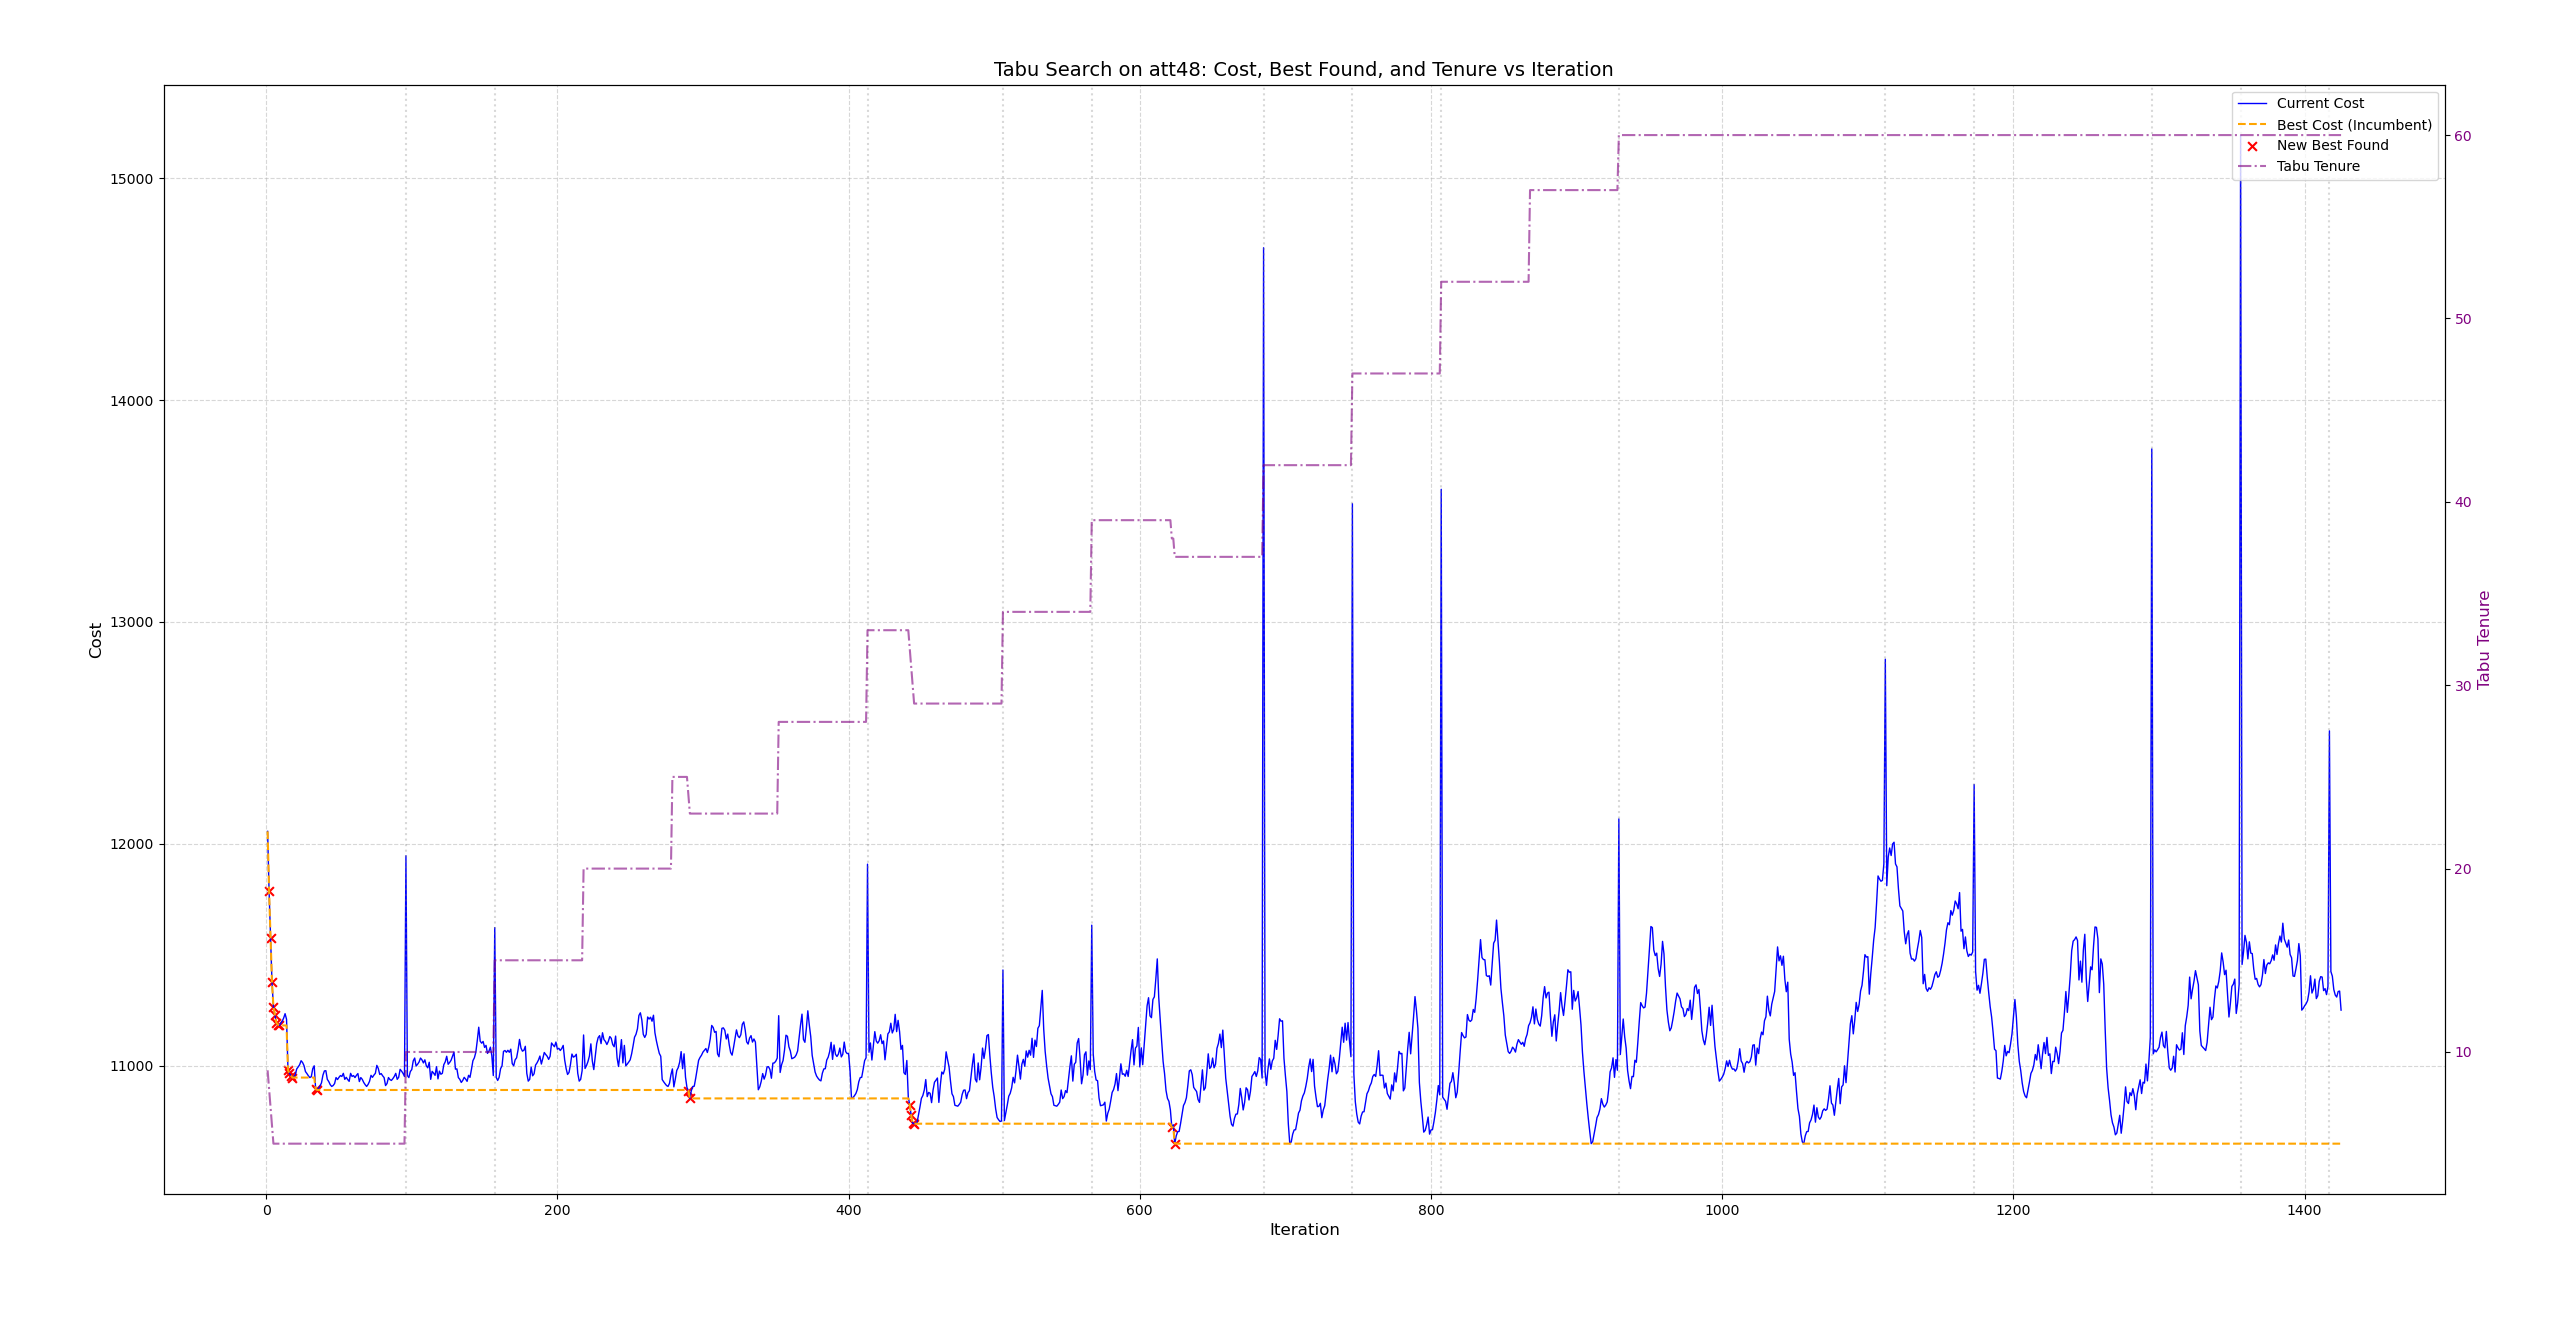
\includegraphics[width=\textwidth]{images/tabu_run_att48.png}
    \caption{Evolution of solution cost (blue), best solution found (orange), and tabu tenure (purple, right axis) across iterations for Tabu Search on \texttt{att48}. Red crosses indicate when a new best solution was discovered.}
    \label{fig:tabu_plot}
\end{figure}

\clearpage

\section{Variable Neighborhood Search (VNS)}

A known limitation of the Tabu Search algorithm is the need to carefully tune several hyperparameters, such as the size and policy 
of the tabu list (static or dynamic tenure), which may be unaffordable in real-world scenarios and can lead to overfitting. 
Furthermore, diversification steps in Tabu Search might waste computational resources without significantly improving solution quality.

A simpler alternative is the \textit{Variable Neighborhood Search (VNS)} metaheuristic~\cite{Hansen2009}, 
which addresses the same problem from a different perspective. Rather than maintaining a tabu list to prevent reversals, 
VNS uses random \textit{k-opt} swaps, called \textbf{kicks}, to escape local minima. Since a k-opt move alters more than two edges, 
it is less likely to be undone by a simple 2-opt move.

\subsection{Algorithm Description}

The VNS algorithm iteratively improves a solution using 2-opt until no better neighbor is found. Then, it performs a series of random 3-opt kicks 
to perturb the solution and continues the search. This avoids complete restarts (as in multistart heuristics) and ensures better locality preservation.

The number of kicks is randomly selected within a fixed range $[k_{\text{min}}, k_{\text{max}}]$ and scaled by a learning factor. 
This value is further adjusted based on the number of iterations since the last improvement, allowing the algorithm to increase its exploration 
as it stagnates. This trade-off is analyzed experimentally in Section~\ref{sec:results}.\todo{trade off analysis nella sezione dei rsiultati}

\subsection{3-Opt Kick Structure}

Each kick is implemented as a 3-opt move, which removes three edges and reconnects the resulting segments using one of seven possible reconnection types. 
For each kick, a valid triple of split indices $(i, j, k)$ is selected at random, and all reconnection variants are evaluated. 
The configuration with the lowest cost is retained and applied to the current solution. Figure~\ref{fig:3optkick} illustrates a typical 3-opt transformation.

\begin{figure}[H]
    \centering
    \begin{subfigure}[c]{.4\textwidth}
        \centering
        \resizebox{\linewidth}{!}{
            \begin{tikzpicture}
                \begin{scope}[every node/.style={circle,thick,draw}]
                    \node (I) at (2.5,4) {$p_i$};
                    \node (II) at (0,3) {$p_{i+1}$};
                    \node (J) at (0,0) {$p_j$};
                    \node (JJ) at (2,-1) {$p_{j+1}$};
                    \node (K) at (4.5,0.3) {$p_k$};
                    \node (KK) at (4.5,2.7) {$p_{k+1}$};
                \end{scope}

                \begin{scope}[>={Stealth[black]}, every node/.style={fill=white,circle},
                            every edge/.style={draw=red,very thick}]
                    \path[->] (I) edge[draw=black] (II);
                    \path[->] (J) edge[draw=black] (JJ);
                    \path[->] (K) edge[draw=black] (KK);
                    \path[->] (II) edge[dashed, draw=black, thin, bend right=40] (J);
                    \path[->] (JJ) edge[dashed, draw=black, thin, bend right=40] (K);
                    \path[->] (KK) edge[dashed, draw=black, thin, bend right=40] (I);
                \end{scope}
            \end{tikzpicture}
        }
    \end{subfigure}
    \hspace{1em}
    \raisebox{-0.5\height}{$\Rightarrow$}
    \hspace{1em}
    \begin{subfigure}[c]{.4\textwidth}
        \centering
        \resizebox{\linewidth}{!}{
            \begin{tikzpicture}
                \begin{scope}[every node/.style={circle,thick,draw}]
                    \node (I) at (2.5,4) {$p_i$};
                    \node (II) at (0,3) {$p_{i+1}$};
                    \node (J) at (0,0) {$p_j$};
                    \node (JJ) at (2,-1) {$p_{j+1}$};
                    \node (K) at (4.5,0.3) {$p_k$};
                    \node (KK) at (4.5,2.7) {$p_{k+1}$};
                \end{scope}

                \begin{scope}[>={Stealth[black]}, every node/.style={fill=white,circle},
                            every edge/.style={draw=red,very thick}]
                    \path[->] (I) edge[draw=blue] (K);
                    \path[->] (JJ) edge[draw=blue] (II);
                    \path[->] (J) edge[draw=blue] (KK);
                    \path[->] (II) edge[dashed, draw=black, thin, bend right=40] (J);
                    \path[->] (K) edge[dashed, draw=blue, bend left=40] (JJ);
                    \path[->] (KK) edge[dashed, draw=black, thin, bend right=40] (I);
                \end{scope}
            \end{tikzpicture}
        }
    \end{subfigure}
    \caption{Effect of a 3-opt kick applied to a TSP tour.}
    \label{fig:3optkick}
\end{figure}

\subsection{Pseudocode}

\begin{algorithm}[H]
\caption{VNS high-level pseudocode}
\label{alg:vns_highlevel}
\begin{algorithmic}
\State \textbf{Input:} Instance \texttt{inst}, initial solution \texttt{sol}
\State \textbf{Output:} Best solution found
\State
\If{solution not initialized}
    \State Generate initial path (greedy or random)
\EndIf
\While{time not exceeded}
    \State Apply 2-opt to refine \texttt{sol}
    \If{\texttt{sol} improves}
        \State Update best known solution
    \Else
        \State Compute number of 3-opt kicks (based on $[k_{\min}, k_{\max}]$, learning rate, stagnation)
        \For{each kick}
            \State Apply 3-opt with best of 7 reconnection types
        \EndFor
    \EndIf
\EndWhile
\State \Return best solution found
\end{algorithmic}
\end{algorithm}


\subsection{Search Behavior Analysis}

To better understand the internal dynamics of the VNS algorithm, we tracked the solution cost, number of 3-opt kicks applied, and moments when new best solutions were discovered. Figure~\ref{fig:vns_plot} shows a representative run on the \texttt{att48} instance. This execution was deliberately performed with a reduced time limit in order to produce a visually rich and interpretable trace of the algorithm's behavior over a large number of iterations. The results should therefore be interpreted qualitatively rather than quantitatively.

\begin{figure}[H]
    \centering
    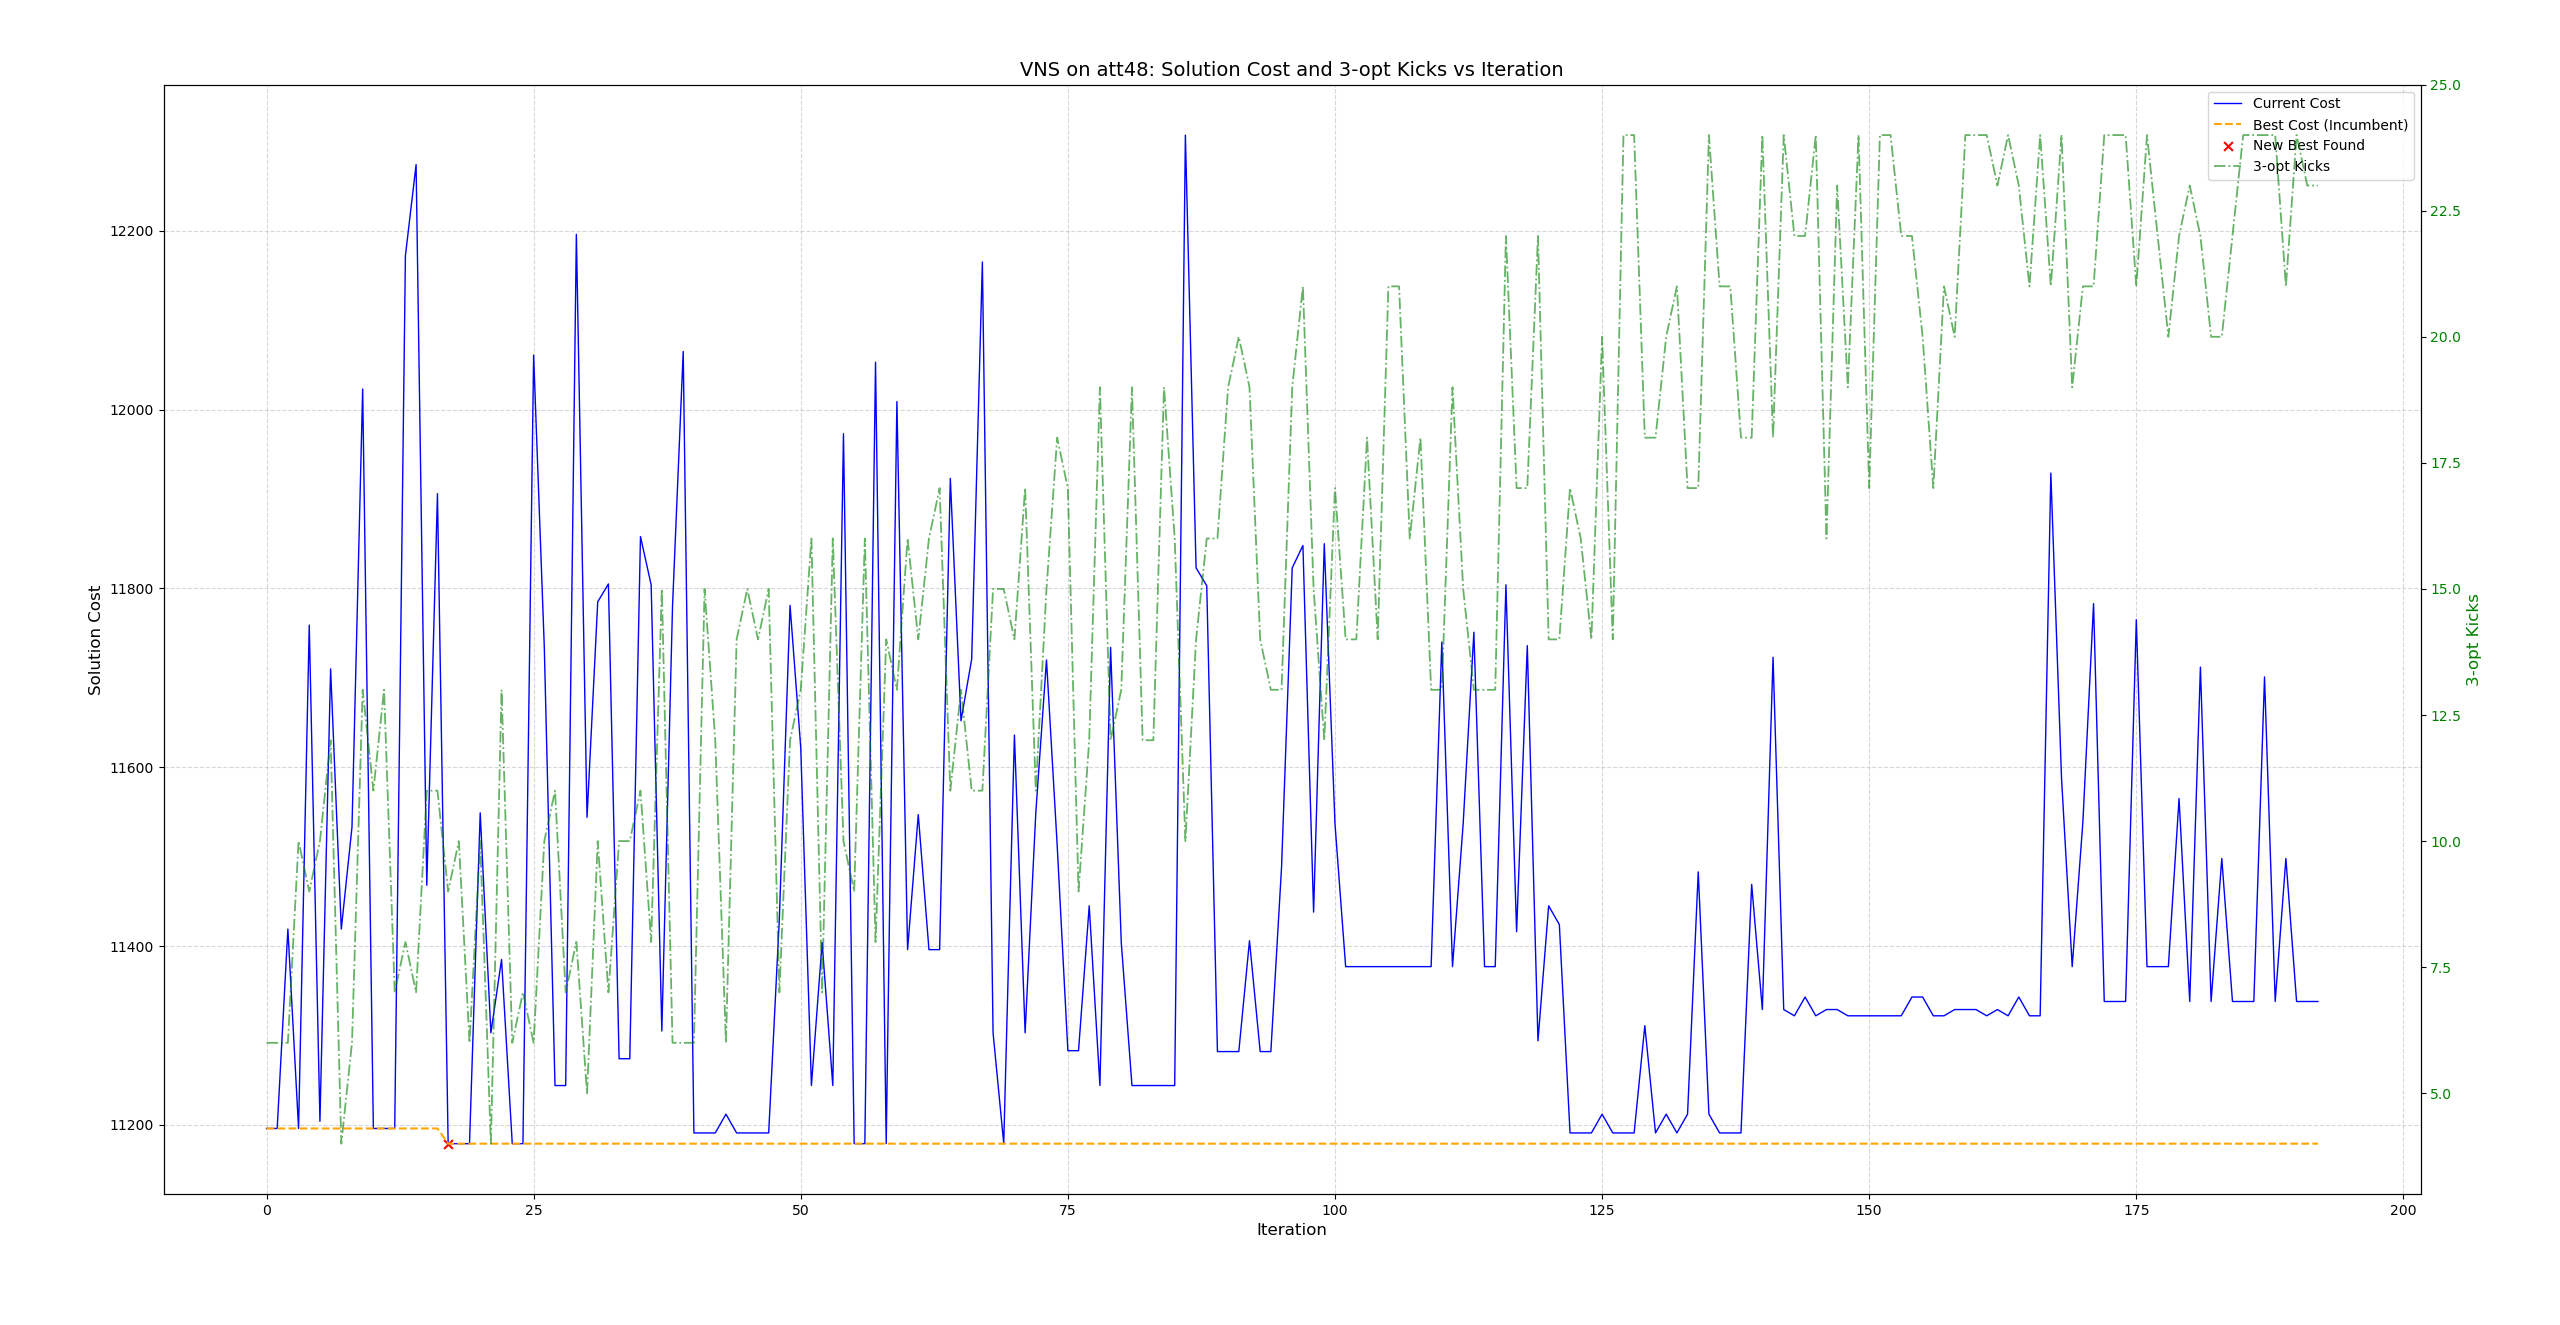
\includegraphics[width=\textwidth]{images/vns_run_att48.png}
    \caption{Evolution of solution cost (blue), best solution found (orange), and number of 3-opt kicks (green, right axis) across iterations for VNS on \texttt{att48}. Red crosses indicate new best solutions.}
    \label{fig:vns_plot}
\end{figure}

As the plot illustrates, the algorithm alternates between local refinement phases using 2-opt and diversification phases driven by a variable number of 3-opt kicks. The current solution cost (blue) exhibits significant fluctuation, especially during early iterations, as the algorithm explores different regions of the solution space. These fluctuations are a natural consequence of aggressive perturbations, which often increase the solution cost before re-converging toward local optima.

The number of 3-opt kicks applied (green, right axis) tends to grow over time as the algorithm adapts to longer periods without improvement. 
This allows for progressively broader exploration of the solution space. Periodic improvements to the best solution (orange), marked by red crosses, 
highlight successful escapes from local minima.

While this run was not intended to produce optimal results, it clearly shows the iterative interaction between intensification and diversification mechanisms that define the VNS approach.
